\RequirePackage[l2tabu, orthodox]{nag}
\documentclass{article}

\newcounter{chapter}
\setcounter{chapter}{3} % Modify Counter To Chapter

\setcounter{section}{\value{chapter}}
\addtocounter{section}{-1}

\usepackage{amssymb,amsmath,verbatim,graphicx,microtype,units,booktabs}
\usepackage[margin=10pt, font=small, labelfont=bf, labelsep=endash]{caption}
\usepackage[colorlinks=true, pdfborder={0 0 0}]{hyperref}
\usepackage[utf8]{inputenc}
\usepackage{pdfpages}

\usepackage[left=0.75in, right=0.75in]{geometry}
\usepackage{titleps}
\newpagestyle{main}{
    \setheadrule{.4pt}
    \sethead{Chapter \thechapter: \sectiontitle}
            {}
            {Illya Starikov}
}
\pagestyle{main}

\begin{document}
\section{The Biological Bases of Behavior}

\subsection{Study Guide Material}
\begin{description}
    \item [left brain/right brain]
    \item [depression]
    \item [neurons] individual cells in the nervous system that receive, integrate, and transmit information.
    \item [acetylcholine]
    \item [dopamine]
    \item [norepinephrine]
    \item [GABA] Another group of transmitters consists of amino acids. One transmitter in this group, gamma-aminobutyric acid (GABA), is notable in that it seems to produce only inhibitorypostsynaptic potentials. Some transmitters, such as ACh and NE, are versatile. They can produce either excitatory or inhibitory PSPs, depending on the synaptic receptors they bind to. However, GABA appears to have inhibitory effects at virtually all synapses where it is present. GABA receptors are widely distributed in the brain and may be present at 40\% of all synapses. GABA appears to be responsible for much of the inhibition in the central nervous system. Studies suggest that GABA is involved in the regulation of anxiety in humans and that disturbances in GABA circuits may contribute to some types of anxiety disorders (Garakani et al., 2009). GABA circuits also play a central role in the expression of some types of seizures (Shank, Smith-Swintosky,\& Twyman, 2000), and they contribute to the modulation of sleep (Siegel, 2004).
    \item [Pituitary] Master Gland!
    \item [Glutamate]
    \item [Endorphins]
    \item [Peripheral nervous system]
    \item [Spinal cord]
    \item [Hindbrain]
    \item [Cerebellum]
    \item [Forebrain] has four main things responsible for --- and it's the largest!
    \begin{enumerate}
        \item Thalamus: Sensory infromation
        \item Hypothalamus: the four Fs: fight, flight, feeding, mating
        \item Limbic system: Pleasure
        \item Cerebrum: learning
    \end{enumerate}
    \item [Hippocampus]
    \item [Hormones]
    \item [Testosterone] Linked to aggression. Steroid hormone from the androgen group and is found in humans and other vertebrates. In humans and other mammals, testosterone is secreted primarily by the testicles of males and, to a lesser extent, the ovaries of females.
    \item [Oxytocin] love hormone.
    \item [Charles Darwin] Father of evolution. Proposed survival of the fittest. Natural selection will weed out the weak, the strongest will survive.
\end{description}


\subsection{Book Notes}
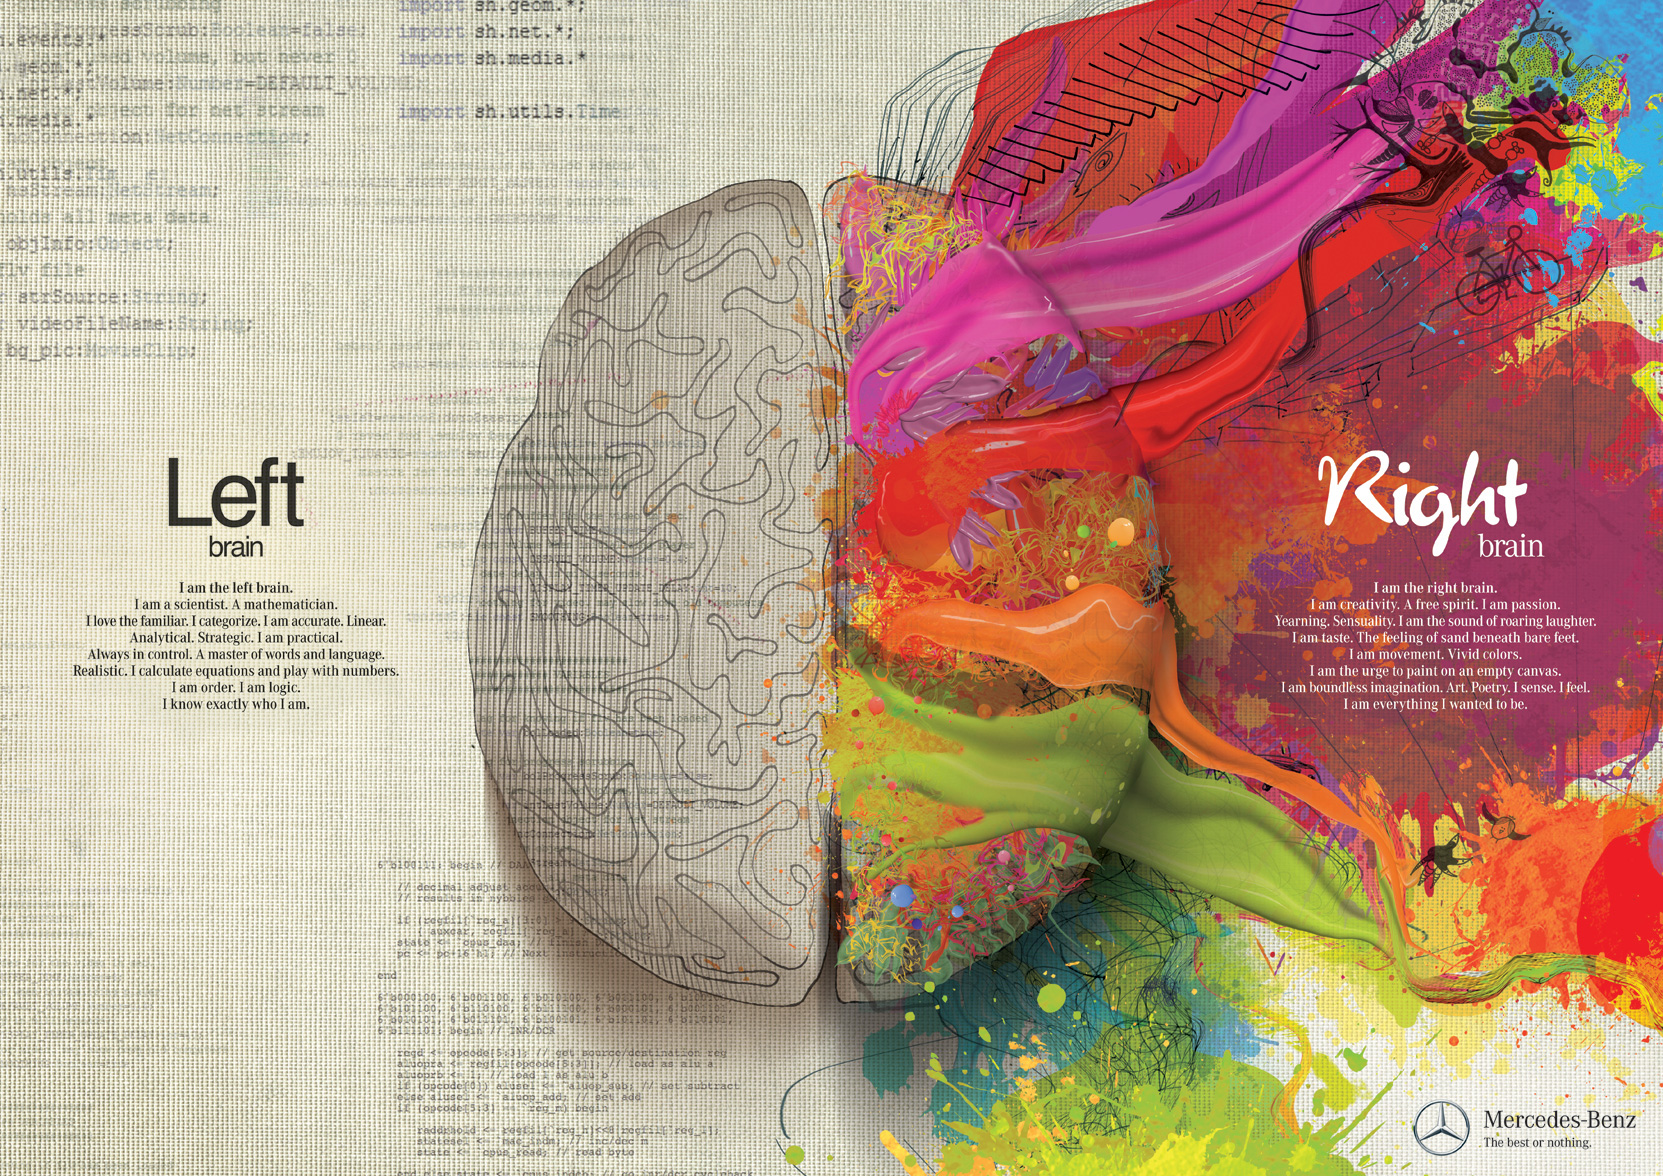
\includegraphics[width=\textwidth]{brain_sides.jpg}
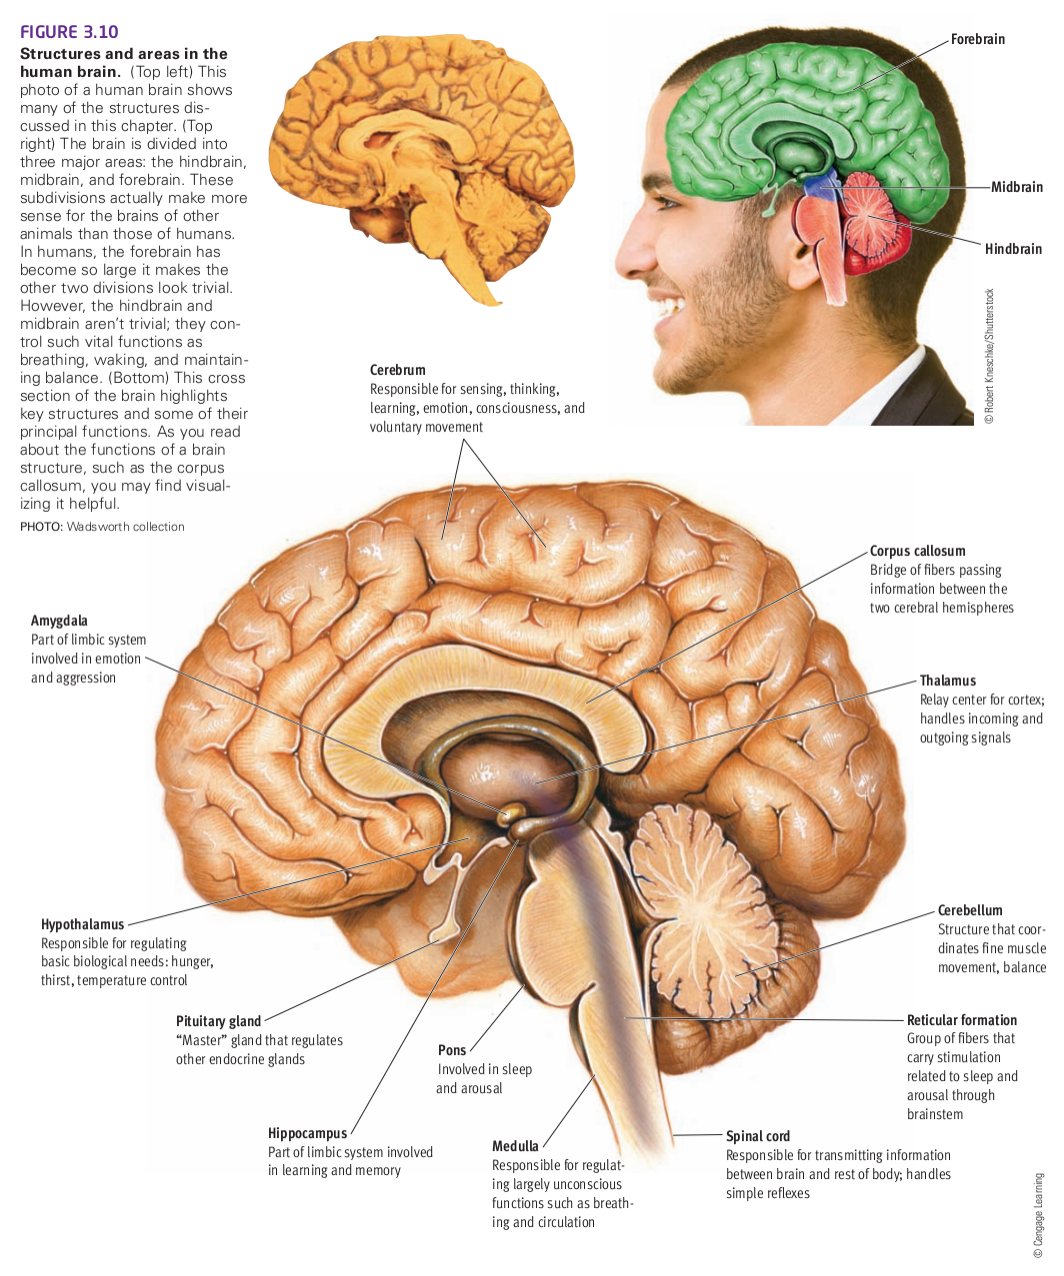
\includegraphics[width=\textwidth]{brain}
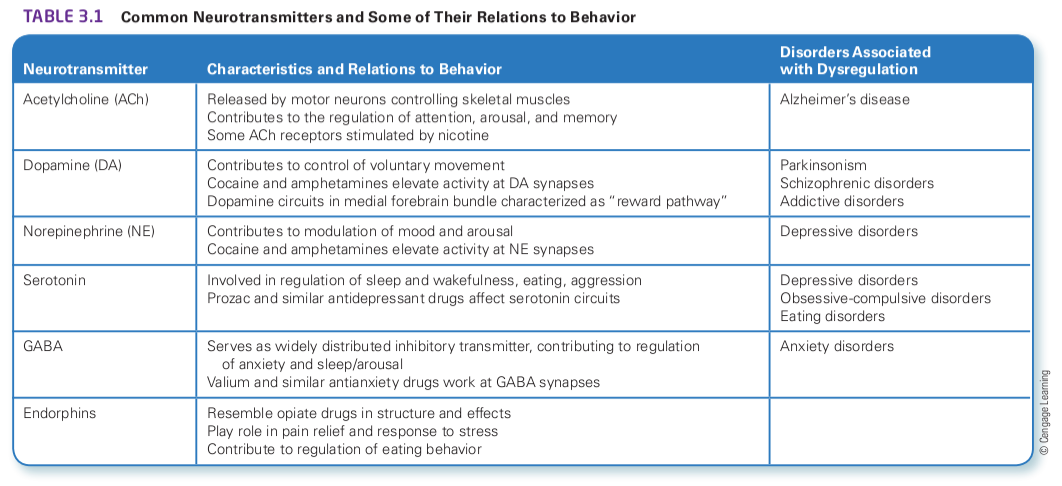
\includegraphics[width=\textwidth]{neurotransmitters}

\subsection{Powerpoint Notes}
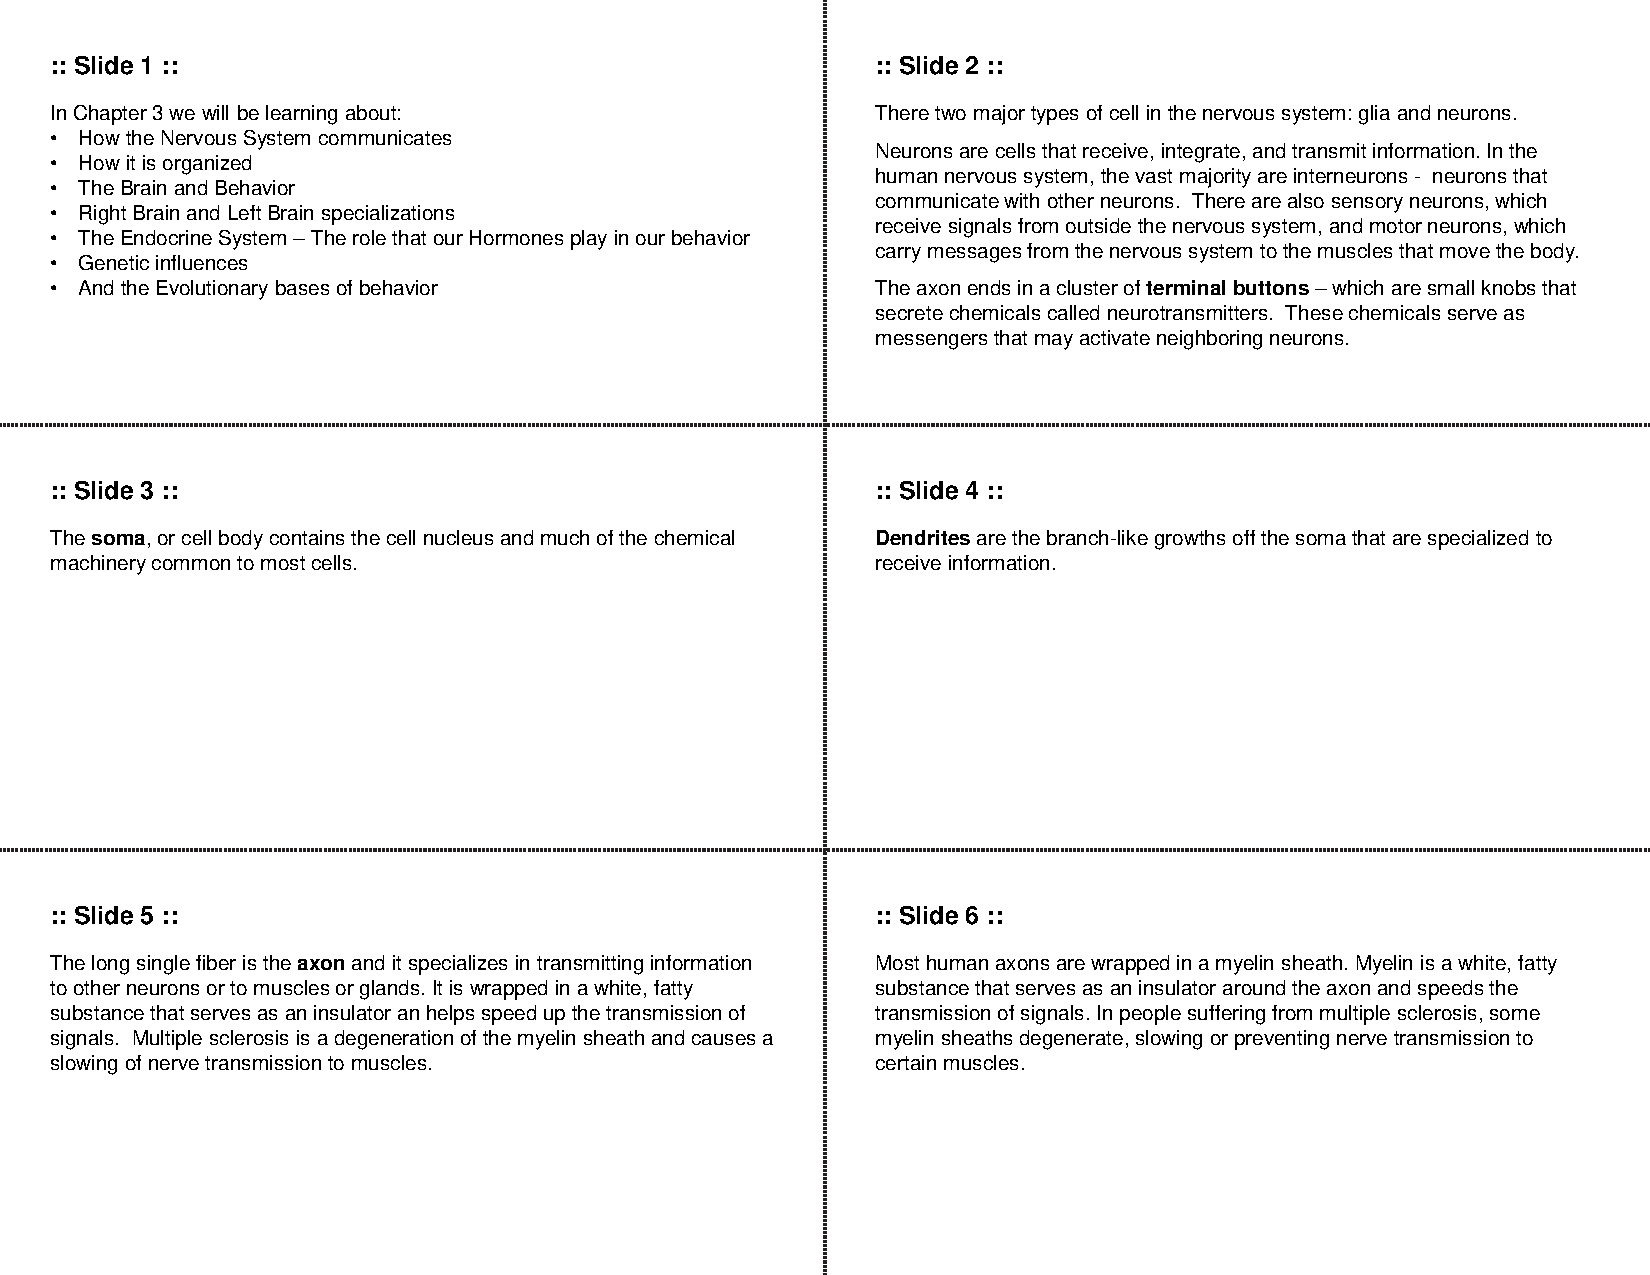
\includepdf[width=1.15\textwidth, pages=-]{lecture_notes.pdf}

\end{document}